\documentclass[11pt]{book}
\usepackage{mathtools}
\usepackage{amsthm, amssymb, amsmath}
\usepackage{graphicx}
\usepackage{subcaption}
\usepackage{amssymb}
\usepackage{microtype}

\newtheorem{thm}{Theorem}[section]
\newtheorem{prop}[thm]{Proposition}
\newtheorem{cor}[thm]{Corollary}
\theoremstyle{definition}
\newtheorem{defn}[thm]{Definition}

\numberwithin{equation}{section}

\usepackage[hidelinks]{hyperref}

\begin{document}

\title{Mathematical Foundations of SigAlg}
\author{John Myers}

\maketitle

\tableofcontents

\chapter{Measure-theoretic probability theory}

\section{\texorpdfstring{$\sigma$-algebras and probability spaces}{Sigma-algebras and probability spaces}}

\subsection{\texorpdfstring{$\sigma$-algebras}{Sigma-algebras}}

\begin{defn}
	Let $\Omega$ be a finite set. A \textit{$\sigma$-algebra} on $\Omega$ is a collection $\mathcal{F}$ of subsets of $\Omega$ with the following properties:
	\begin{enumerate}
		\item The set $\Omega$ itself is contained in $\mathcal{F}$.
		\item If $U$ is a set in $\mathcal{F}$, then the complement $U^c = \Omega \smallsetminus U$ is also in $\mathcal{F}$.
		\item If both $U$ and $V$ are sets in $\mathcal{F}$, then the union $U\cup V$ is also in $\mathcal{F}$.
	\end{enumerate}
	A set in $\mathcal{F}$ is called an \textit{$\mathcal{F}$-measurable set}, or simply a \textit{measurable set} if the identity of the $\sigma$-algebra is clear. In the probabilistic context, measurable sets are called \textit{events}.
\end{defn}

\begin{defn}
	A \textit{finite measurable space} is a pair $(\Omega, \mathcal{F})$ consisting of a finite set $\Omega$ and a $\sigma$-algebra $\mathcal{F}$ on $\Omega$.
\end{defn}

\begin{defn}
	Let $\mathcal{F}$ and $\mathcal{G}$ be two $\sigma$-algebras on a finite set $\Omega$. If $\mathcal{G} \subset \mathcal{F}$, we say $\mathcal{G}$ is a \textit{sub-$\sigma$-algebra} of $\mathcal{F}$ (or that $\mathcal{G}$ is \textit{coarser} than $\mathcal{F}$), and that $\mathcal{F}$ is a \textit{super-$\sigma$-algebra} of $\mathcal{G}$ (or that $\mathcal{F}$ is \textit{finer} than $\mathcal{G}$).
\end{defn}

\begin{defn}
	Let $\mathcal{F}$ be a $\sigma$-algebra on a finite set $\Omega$. An \textit{atom} of $\mathcal{F}$ is a set $A$ in $\mathcal{F}$ with the following two properties:
	\begin{enumerate}
		\item It is nonempty, $A\neq \emptyset$.
		\item If $B$ is a nonempty set in $\mathcal{F}$ with $B\subset A$, then $A=B$.
	\end{enumerate}
	The set of all atoms of $\mathcal{F}$ will be denoted $\alpha(\mathcal{F})$.
\end{defn}

\begin{thm}[Atomic Partition Theorem]
	Let $\Omega$ be a finite set. There is a bijective correspondence between the collection of $\sigma$-algebras on $\Omega$ and the collection of partitions, given as follows:
	\begin{enumerate}
		\item Every $\sigma$-algebra $\mathcal{F}$ on $\Omega$ yields a partition of $\Omega$, where the sets in the partition are the atoms of $\mathcal{F}$.
		\item Every partition of $\Omega$ yields a $\sigma$-algebra $\mathcal{F}$ on $\Omega$, where the sets in $\mathcal{F}$ are all unions of sets in the partition, along with $\emptyset$.
	\end{enumerate}
\end{thm}

\subsection{\texorpdfstring{Lattices of $\sigma$-algebras}{Lattices of sigma-algebras}}

\subsection{Probability spaces}

\begin{defn}
	Let $\mathcal{F}$ be a $\sigma$-algebra on a finite set $\Omega$.
	\begin{enumerate}
		\item A \textit{measure} on $\mathcal{F}$ is a function $\mu:\mathcal{F} \to [0,\infty)$ with the following property: If $U$ and $V$ are two $\mathcal{F}$-measurable sets that are disjoint, then $\mu(U\cup V) = \mu(U) + \mu(V)$.
		\item Suppose $\Omega$ is nonempty. A \textit{probability measure} on $\mathcal{F}$ is a measure $P: \mathcal{F} \to [0,\infty)$ such that $P(\Omega)=1$.
	\end{enumerate}
\end{defn}

\begin{defn}
	\leavevmode
	\begin{enumerate}
		\item A \textit{finite measure space} is a triple $(\Omega, \mathcal{F}, \mu)$ consisting of a finite set $\Omega$, a $\sigma$-algebra $\mathcal{F}$ on $\Omega$, and a measure $\mu$ on $\mathcal{F}$.
		\item A \textit{finite probability space} is a triple $(\Omega, \mathcal{F}, P)$ consisting of a finite, nonempty set $\Omega$, a $\sigma$-algebra $\mathcal{F}$ on $\Omega$, and a probability measure $P$ on $\mathcal{F}$.
	\end{enumerate}
\end{defn}

\section{Functions and integration}

\subsection{Random variables and vectors}

\begin{defn}
	Let $(\Omega, \mathcal{F})$ be a finite measurable space and $d$ a positive integer. A function $\mathbf{X}: \Omega \to \mathbb{R}^d$ is called \textit{$\mathcal{F}$-measurable} if the preimage
	\[
		\{\mathbf{X} = \mathbf{x}\} \stackrel{\text{def}}{=} \{ \omega \in \Omega : \mathbf{X}(\omega)=\mathbf{x}\}
	\]
	is in $\mathcal{F}$, for each $\mathbf{x}\in \mathbb{R}^d$. If the identity of the $\sigma$-algebra is clear from context, \textit{$\mathcal{F}$-measurable} will be shortened to just \textit{measurable}.
\end{defn}

\begin{defn}
	Let $(\Omega, \mathcal{F})$ be a finite measurable space.
	\begin{enumerate}
		\item A \textit{$d$-dimensional random vector} is an $\mathcal{F}$-measurable function $\mathbf{X}: \Omega \to \mathbb{R}^d$.
		\item A \textit{random variable} is a $1$-dimensional random vector, i.e., an $\mathcal{F}$-measurable function $X: \Omega \to \mathbb{R}$.
	\end{enumerate}
\end{defn}

\begin{thm}[Atomic Criterion for Measurability]\label{thm:atomic-criterion-measurable}
	Let $(\Omega, \mathcal{F})$ be a finite measurable space. A function $\mathbf{X}: \Omega \to \mathbb{R}^d$ is $\mathcal{F}$-measurable (i.e., it is a random vector) if and only if it is constant on the atoms of $\mathcal{F}$.
\end{thm}

\begin{defn}
	Let $\Omega$ be a finite set and $\mathbf{X}: \Omega \to \mathbb{R}^d$ a function. The \textit{$\sigma$-algebra generated by $\mathbf{X}$}, denoted $\sigma(\mathbf{X})$, is the $\sigma$-algebra on $\Omega$ whose atoms are the nonempty preimages $\{\mathbf{X} = \mathbf{x}\}$, one for each vector $\mathbf{x}\in \mathbb{R}^d$ for which the preimage is nonempty.
\end{defn}

\begin{thm}[Functional Criterion for Measurability]\label{thm:functional-criterion-measurable}
	Let $\Omega$ be a finite set and let $\mathbf{X}: \Omega \to \mathbb{R}^d$ be a function. Then a function $\mathbf{Y}: \Omega \to \mathbb{R}^e$ is $\sigma(\mathbf{X})$-measurable if and only if there is a function $h: \mathbb{R}^d \to \mathbb{R}^e$ such that $\mathbf{Y} = h(\mathbf{X})$.
\end{thm}

This is a key result, so it deserves elaboration. Supposing that $\mathbf{Y}$ is $\sigma(\mathbf{X})$-measurable, a function $h$ as in the theorem is constructed as follows. If $\mathbf{x}\in \mathbb{R}^d$ is a vector whose preimage $\{\mathbf{X} = \mathbf{x}\}$ is nonempty, we define
\[
	h(\mathbf{x}) = \mathbf{Y}(\{\mathbf{X} = \mathbf{x}\}),
\]
where the right-hand side is the unique value of $\mathbf{Y}$ on the preimage $\{\mathbf{X} = \mathbf{x}\}$. For those vectors $\mathbf{x}\in \mathbb{R}^d$ such that $\{\mathbf{X} = \mathbf{x}\}$ is empty, we define $h(\mathbf{x})$ to be an arbitrary but fixed value. Note that the only part of $h$ that is unique is its restriction to the range of $\mathbf{X}$.

\begin{thm}[Universal property of generated $\sigma$-algebras]
	Let $\Omega$ be a finite set and $\mathbf{X}: \Omega \to \mathbb{R}^d$ a function.
	\begin{enumerate}
		\item The function $\mathbf{X}$ is $\sigma(\mathbf{X})$-measurable.
		\item If $\mathcal{F}$ is a $\sigma$-algebra on $\Omega$ for which $\mathbf{X}$ is $\mathcal{F}$-measurable, then $\sigma(\mathbf{X}) \subset \mathcal{F}$.
	\end{enumerate}
\end{thm}

\subsection{Integration and expectation}

Let $X$ be a random variable on a finite measurable space $(\Omega, \mathcal{F})$. Given an atom $A$ of $\mathcal{F}$, by Theorem \ref{thm:atomic-criterion-measurable} the value $X(\omega)$ is constant as $\omega$ ranges over $A$. We write $X(A)$ for this unique value.

\begin{defn}
	Let $X$ be a random variable on a finite probability space $(\Omega, \mathcal{F}, P)$. Given an event $U\in \mathcal{F}$, we define the \textit{Lebesgue integral} of $X$ over $U$ to be the real number
	\[
		\int_U X \, dP = \sum_{A\in \alpha(\mathcal{F})} I_U(A)X(A)P(A),
	\]
	where $I_U$ is the indicator function of $U$.
\end{defn}

\begin{defn}
	Let $X$ be a random variable on a finite probability space $(\Omega, \mathcal{F}, P)$. The \textit{expected value} of $X$, denoted $E(X)$, is the real number
	\[
		E(X) = \int_\Omega X \, dP.
	\]
\end{defn}

\begin{thm}[Properties of the Lebesgue integral]\label{thm:integral-properties}
	Let $(\Omega, \mathcal{F}, P)$ be a finite probability space, let $X, Y$ be random variables on $\Omega$, let $U, V \in \mathcal{F}$, and let $a, b \in \mathbb{R}$.
	\begin{enumerate}
		\item (\textit{Linearity})
		      \[
			      \int_U (aX + bY) \, dP = a \int_U X \, dP + b \int_U Y \, dP.
		      \]
		\item (\textit{Monotonicity}) If $X(\omega) \leq Y(\omega)$ for all $\omega \in U$, then
		      \[
			      \int_U X \, dP \leq \int_U Y \, dP.
		      \]
		\item (\textit{Additivity over domains}) If $U$ and $V$ are disjoint, then
		      \[
			      \int_{U \cup V} X \, dP = \int_U X \, dP + \int_V X \, dP.
		      \]
		\item (\textit{Constants}) If $X$ is the constant random variable equal to $c \in \mathbb{R}$, then
		      \[
			      \int_U X \, dP = c \, P(U).
		      \]
		\item (\textit{Indicators})
		      \[
			      \int_\Omega I_U \, dP = P(U).
		      \]
		\item (\textit{Triangle inequality})
		      \[
			      \left| \int_U X \, dP \right| \leq \int_U |X| \, dP.
		      \]
	\end{enumerate}
\end{thm}



\section{\texorpdfstring{$L^2$-spaces}{L2-spaces}}

Many constructs in measure-theoretic probability theory are clarified through the introduction of a geometric viewpoint. This geometry comes through the Hilbert space structure on sets of random variables that we introduce in:

\begin{defn}\label{defn:l2}
	Letting $(\Omega, \mathcal{F}, P)$ be a finite probability space, we write $L^2(\Omega, \mathcal{F}, P)$ for the set of all $\mathcal{F}$-measurable random variables on $\Omega$.
	\begin{enumerate}
		\item We define the \textit{sum} of two random variables $X$ and $Y$ in $L^2(\Omega, \mathcal{F}, P)$, denoted $X+Y$, to be the $\mathcal{F}$-measurable random variable given by
		      \[
			      (X+Y)(\omega) = X(\omega) + Y(\omega),
		      \]
		      for all $\omega \in \Omega$. We define the \textit{product} of $X$ and $Y$, denoted $XY$, to be the $\mathcal{F}$-measurable random variable given by
		      \[
			      (XY)(\omega) = X(\omega) Y(\omega),
		      \]
		      for all $\omega\in \Omega$. Given a scalar $c\in \mathbb{R}$, we define the \textit{scalar multiple} of $c$ and $X$, denoted $cX$, to be the $\mathcal{F}$-measurable random variable given by
		      \[
			      (cX)(\omega) = c X(\omega),
		      \]
		      for all $\omega \in \Omega$. Finally, we define the \textit{zero random variable} to be the constant random variable that sends every $\omega\in \Omega$ to $0\in \mathbb{R}$.
		\item We define the \textit{inner product} of two random variables $X$ and $Y$ in $L^2(\Omega, \mathcal{F}, P)$, denoted $\langle X, Y \rangle$, to be the real number given by
		      \[
			      \langle X, Y\rangle = \int_\Omega XY \, dP.
		      \]
	\end{enumerate}
\end{defn}

Our definition of $H = L^2(\Omega, \mathcal{F}, P)$ as a set of \textit{actual} random variables presents a difficulty of what it should mean for two random variables in $H$ to be \textit{equal}. For example, suppose that $N$ is a set in $\mathcal{F}$ with zero probability, $P(N)=0$, and suppose that $X\in H$ is a random variable which is equal to $0$ on the complement $N^c$, but takes a nonzero value on $N$. Then $X$ is not equal to the zero random variable in $H$, but yet
\[
	\int_\Omega X \, dP=0.
\]
As we will see in Theorem \ref{thm:hilbert} below, this will mean that the inner product given in Definition \ref{defn:l2} is \textit{not} positive definite.

However, notice that $X$ is \textit{almost surely equal} to the zero random variable, in the following sense:

\begin{defn}
	Let $X$ and $Y$ be two random variables on a finite probability space $(\Omega, \mathcal{F}, P)$. Then $X$ and $Y$ are \textit{almost surely equal} if the set
	\[
		N = \{\omega \in \Omega \mid X(\omega) \neq Y(\omega) \}
	\]
	has probability $0$.
\end{defn}

There are then two ways to leverage this notion of \textit{almost sure equality} in a proper definition of the space $H = L^2(\Omega, \mathcal{F},P)$. First, instead of defining $H$ to be a set of actual random variables, one can define it as the set of equivalence classes of random variables, where the equivalence relation is almost sure equality. Strictly speaking, this is the proper definition. Alternatively, one can keep $H$ as a set of random variables, and just understand that equality of random variables in $H$ really means almost sure equality. This latter road is the one we take.

It will be convenient to write $\alpha'(\mathcal{F})$ for the subset of $\alpha(\mathcal{F})$ consisting of all atoms of nonzero probability.

With this convention in force, we then have the main theorem:

\begin{thm}[Algebro-geometric structure of $L^2$-spaces]\label{thm:hilbert}
	Let $(\Omega, \mathcal{F}, P)$ be a finite probability space and set $H = L^2(\Omega, \mathcal{F}, P)$.
	\begin{enumerate}
		\item Equipped with the sum, scalar multiplication, and zero random vector defined in Definition \ref{defn:l2}, the set $H$ is a finite-dimensional vector space.
		\item Equipped with the vector space structure in (1) and the inner product defined in Definition \ref{defn:l2}, the set $H$ is a Hilbert space.
		\item The Hilbert space $H$ has an orthogonal basis consisting of all indicator functions $I_A$, as $A$ ranges over the set $\alpha'(\mathcal{F})$ of all atoms of $\mathcal{F}$ with nonzero probability.
	\end{enumerate}
\end{thm}

We compute an \textit{orthonormal} basis by normalizing the indicator functions in the orthogonal basis identified in the theorem. For this, we use the following computation:
\[
	\| I_A \|^2 = \langle I_A, I_A \rangle = \int_\Omega I_A^2 \, dP = P(A).
\]
Thus, the space $H$ has an orthonormal basis consisting of all scaled indicator functions
\begin{equation}\label{eq:onb}
	\phi_A \stackrel{\text{def}}{=} \frac{I_A}{\sqrt{P(A)}},
\end{equation}
one for each atom $A\in \alpha'(\mathcal{F})$.

Suppose that $K$ is a vector subspace of $H$. Given a random variable $X\in H$, the \textit{orthogonal projection of $X$ onto $K$} is the unique random variable $\Pi$ such that $\Pi\in K$ and $\langle \Pi-X, Y \rangle = 0$ for all $Y\in K$. If $K$ has an orthonormal basis $\{Y_i\}_{i\in I}$, then $\Pi$ is given by its \textit{generalized Fourier expansion}:
\begin{equation}\label{eq:fourier}
	\Pi = \sum_{i\in I} \langle X, Y_i \rangle Y_i.
\end{equation}
Important examples of subspaces are of the form $K = L^2(\Omega, \mathcal{G}, P|_{\mathcal{G}})$, where $\mathcal{G}$ is a sub-$\sigma$-algebra of $\mathcal{F}$ and $P|_{\mathcal{G}}: \mathcal{G} \to [0,\infty)$ is the restriction of $P$ to $\mathcal{G}$. Orthogonal projections onto subspaces of this type have special names:

\begin{defn}
	Let $X$ be a random variable on a finite probability space $(\Omega, \mathcal{F}, P)$, and let $\mathcal{G}$ be a sub-$\sigma$-algebra of $\mathcal{F}$. The \textit{conditional expectation of $X$ given $\mathcal{G}$}, denoted $E(X \mid \mathcal{G})$, is the orthogonal projection of $X$ onto the subspace $L^2(\Omega, \mathcal{G}, P|_{\mathcal{G}})$.
\end{defn}

Using the orthonormal basis of $K=L^2(\Omega, \mathcal{G}, P|_{\mathcal{G}})$ consisting of scaled indicator functions \eqref{eq:onb}, conditional expectations may be computed using their Fourier expansions \eqref{eq:fourier}. To do so, let an atom $B\in \alpha'(\mathcal{G})$ be given and consider the basis random vector $\phi_B$. We have
\[
	\langle X, \phi_B \rangle \phi_B = \frac{\int_B X \, dP}{P(B)}  I_B,
\]
and so
\[
	E(X \mid \mathcal{G}) = \sum_{B \in \alpha'(\mathcal{G})} \frac{\int_B X \, dP}{P(B)}  I_B.
\]

Directly from the definition of a conditional expectation as an orthogonal projection, one proves:

\begin{thm}[Uniqueness of conditional expectations]\label{thm:orthogonality-cond-exp}
	Let $X$ be a random variable on a finite probability space $(\Omega, \mathcal{F}, P)$, and let $\mathcal{G}$ be a sub-$\sigma$-algebra of $\mathcal{F}$.
	\begin{enumerate}
		\item The conditional expectation $E(X\mid \mathcal{G})$ is $\mathcal{G}$-measurable and
		      \[
			      \int_U X \, dP = \int_U E(X\mid \mathcal{G}) \, dP
		      \]
		      for all $U\in \mathcal{G}$.
		\item If $Z$ is another random variable with the two properties of $E(X\mid \mathcal{G})$ listed in (1), then $Z$ and $E(X\mid \mathcal{G})$ are equal almost surely.
	\end{enumerate}
\end{thm}

In some texts on measure-theoretic probability theory, the properties of conditional expectation listed in this latter theorem are taken as the \textit{definition} of conditional expectation.

The characterizing property of conditional expectation as an orthogonal projection makes some of its most useful features easy to establish. We collect the ones we will need most often:

\begin{thm}[Properties of conditional expectations]\label{thm:cond-exp-properties}
	Let $(\Omega, \mathcal{F}, P)$ be a finite probability space, let $X, Y \in L^2(\Omega, \mathcal{F}, P)$, and let $\mathcal{G}$ be a sub-$\sigma$-algebra of $\mathcal{F}$.
	\begin{enumerate}
		\item (\textit{Linearity}) For all $a,b \in \mathbb{R}$,
		      \[
			      E(aX + bY \mid \mathcal{G}) = a\,E(X\mid \mathcal{G}) + b\,E(Y \mid \mathcal{G}).
		      \]
		\item (\textit{Taking out what is known}) If $Y$ is $\mathcal{G}$-measurable, then
		      \[
			      E(XY \mid \mathcal{G}) = Y E(X \mid \mathcal{G}).
		      \]
		\item (\textit{Tower property}) If $\mathcal{H}$ is a sub-$\sigma$-algebra of $\mathcal{G}$, then
		      \[
			      E\big(E(X\mid \mathcal{G}) \mid \mathcal{H}\big) = E(X \mid \mathcal{H}).
		      \]
		\item (\textit{Triviality}) If $\mathcal{G} = \{\emptyset, \Omega\}$ is the trivial $\sigma$-algebra, then $E(X \mid \mathcal{G})$ is the constant random variable equal to $E(X)$.
		\item (\textit{Idempotence}) If $X$ is $\mathcal{G}$-measurable, then $E(X \mid \mathcal{G}) = X$.
	\end{enumerate}
\end{thm}

Each of these properties reflects a familiar fact about orthogonal projections, transplanted to the setting of $H$. For instance, (5) is simply the statement that a vector already lying in a subspace is its own projection onto that subspace, while (3) reflects the fact that $L^2(\Omega,\mathcal{H},P|_{\mathcal{H}})$ is itself a subspace of $L^2(\Omega,\mathcal{G},P|_{\mathcal{G}})$ whenever $\mathcal{H} \subset \mathcal{G}$, so that projecting onto the smaller subspace can be done either directly, or in two stages by way of the larger one.

Suppose that $\mathcal{G}$ is of the special form $\mathcal{G} = \sigma(\mathbf{Y})$, where $\mathbf{Y}$ is a $d$-dimensional $\mathcal{F}$-measurable random vector. Then we write $E(X \mid \mathbf{Y})$ in place of $E(X\mid \sigma(\mathbf{Y}))$. This conditional expectation is $\sigma(\mathbf{Y})$-measurable and so by the Functional Criterion for Measurability (Theorem \ref{thm:functional-criterion-measurable}) there is a function
\begin{equation}\label{eq:cond-exp-func}
	E(X \mid \mathbf{Y} = {?}) :\mathbb{R}^d \to \mathbb{R}, \quad \mathbf{y} \mapsto E(X \mid \mathbf{Y} = \mathbf{y}),
\end{equation}
such that
\[
	E(X \mid \mathbf{Y} = \mathbf{y}) = E(X \mid \mathbf{Y})(\{ \mathbf{Y} = \mathbf{y} \})
\]
for each $\mathbf{y} \in \mathbb{R}^d$ for which $P(\mathbf{Y} = \mathbf{y})>0$. If this probability is $0$, then $E(X\mid \mathbf{Y}=\mathbf{y})=0$. We will show later in Theorem \ref{thm:cond-exp-familiar} that the function $E(X\mid \mathbf{Y} = {?})$ is given by the familiar formula from elementary (i.e., non-measure-theoretic) probability theory.

If $\mathcal{G}$ is of the special form $\mathcal{G} = \sigma(I_U)$, where $I_U$ is the indicator function of an event $U\in \mathcal{G}$, then we shall write $E(X \mid U)$ in place of $E(X \mid \sigma(I_U))$.

Conditional expectations may be used to define another one of the fundamental objects in probability theory:

\begin{defn}
	Let $(\Omega, \mathcal{F}, P)$ be a finite probability space and $\mathcal{G}$ a sub-$\sigma$-algebra of $\mathcal{F}$. The \textit{conditional probability of an event $U\in \mathcal{F}$ given $\mathcal{G}$}, denoted $P(U \mid \mathcal{G})$, is the $\mathcal{G}$-measurable random variable given by
	\[
		P(U \mid \mathcal{G}) = E(I_U \mid \mathcal{G}).
	\]
\end{defn}

Immediately from the definition and Theorem \ref{thm:orthogonality-cond-exp} we get:

\begin{thm}[Uniqueness of conditional probabilities]\label{thm:orthogonality-cond-prop}
	Let $(\Omega, \mathcal{F}, P)$ be a finite probability space, let $\mathcal{G}$ be a sub-$\sigma$-algebra of $\mathcal{F}$, and let $U\in \mathcal{F}$ be an event.
	\begin{enumerate}
		\item The conditional probability $P(U\mid \mathcal{G})$ is $\mathcal{G}$-measurable and
		      \[
			      P(U\cap V) = \int_V P(U\mid \mathcal{G}) \, dP
		      \]
		      for all $V\in \mathcal{G}$.
		\item If $Z$ is another random variable with the two properties of $P(U\mid \mathcal{G})$ listed in (1), then $Z$ and $P(U\mid \mathcal{G})$ are equal almost surely.
	\end{enumerate}
\end{thm}


For each atom $B\in \alpha'(\mathcal{G})$, the conditional probability $P(U\mid \mathcal{G})$ is constant on $B$ with value
\[
	P(U\mid \mathcal{G})(B) = \frac{P(U\cap B)}{P(B)}.
\]
For a such an atom, the mapping
\[
	P({?}\mid \mathcal{G})(B): \mathcal{F} \to [0, \infty), \quad U \mapsto P(U\mid \mathcal{G})(B),
\]
is a probability measure on the $\sigma$-algebra $\mathcal{F}$.

These measures provide a link with conditional expectations:

\begin{thm}[Conditional expectation via conditional probability]\label{thm:cond-exp-familiar}
	Let $X$ be a random variable on finite probability space $(\Omega, \mathcal{F}, P)$ and let $\mathcal{G}$ be a sub-$\sigma$-algebra of $\mathcal{F}$. Then for all atoms $B\in \alpha(\mathcal{G})$, we have
	\[
		E(X \mid \mathcal{G})(B) = \int_\Omega X \, dP({?} \mid \mathcal{G})(B).
	\]
\end{thm}

In the case that $\mathcal{G} = \sigma(\mathbf{Y})$ for some $d$-dimensional $\mathcal{F}$-measurable random vector $\mathbf{Y}$, we write $P(U \mid \mathbf{Y})$ in place of $P(U \mid \sigma(\mathbf{Y}))$. This conditional probability is a $\sigma(\mathbf{Y})$-measurable random variable, and so by the Functional Criterion for Measurability (Theorem \ref{thm:functional-criterion-measurable}) there is a function
\[
	P(U \mid \mathbf{Y} = {?}): \mathbb{R}^d \to \mathbb{R}, \quad \mathbf{y} \mapsto P(U \mid \mathbf{Y} = \mathbf{y}),
\]
such that
\[
	P(U \mid \mathbf{Y} = \mathbf{y}) = P(U \mid \mathbf{Y})(\{\mathbf{Y} = \mathbf{y}\})
\]
for those vectors $\mathbf{y}\in \mathbb{R}^d$ for which $P(\mathbf{Y} = \mathbf{y})>0$. Unpacking the definitions, we see it is given by the formula
\[
	P(U \mid \mathbf{Y} = \mathbf{y}) = \frac{P\left(U \cap \{\mathbf{Y} = \mathbf{y}\} \right)}{P(\mathbf{Y} = \mathbf{y})}.
\]
If the probability of the preimage $\{\mathbf{Y}=\mathbf{y}\}$ is $0$, then $P(U \mid \mathbf{Y} = \mathbf{y})=0$.

\section{Absolute continuity and Radon-Nikodym derivatives}

\subsection{Absolute continuity}

\begin{defn}
	Let $(\Omega, \mathcal{F})$ be a finite measurable space and $\nu$ and $\mu$ two measures on $\mathcal{F}$. We say that $\nu$ is \textit{absolutely continuous} with respect to $\mu$, written $\mu \ll \mu$,  provided that $\nu(U)=0$ whenever $\mu(U) = 0$, for all $U \in \mathcal{F}$.
\end{defn}

\subsection{Radon-Nikodym derivatives}

\begin{defn}
	Let $(\Omega, \mathcal{F})$ be a finite measurable space and $\nu$ and $\mu$ two measures on $\mathcal{F}$ such that $\nu \ll \mu$. We define a \textit{Radon-Nikodym derivative} of $\nu$ with respect to $\mu$ to be any $\mathcal{F}$-measurable function $h: \Omega \to \mathbb{R}$ for which
	\[
		\nu(U) = \int_U h \, d\mu,
	\]
	for all $U\in \mathcal{F}$.
\end{defn}

The \textit{canonical version} of the Radon-Nikodym of $\nu$ with respect to $\mu$, denoted $d\nu / d\mu$, is given by
\[
	\frac{d\nu}{d\mu}(A) = \begin{cases} \frac{\nu(A)}{\mu(A)} & : \mu(A) \neq 0, \\
	              0                     & : \mu(A) = 0,
	\end{cases}
\]
for all atoms $A\in \alpha(\mathcal{F})$.

\begin{thm}[Change-of-measure formula for Radon-Nikodym derivatives]\label{thm:change-vars}
	Let $(\Omega, \mathcal{F})$ be a finite measurable space and $\nu$ and $\mu$ two measures on $\mathcal{F}$ with $\nu \ll \mu$. Then
	\[
		\int_\Omega f \, d\nu = \int_\Omega f \, \frac{d\nu}{d\mu} \, d\mu
	\]
	for all $\mathcal{F}$-measurable functions $f$.
\end{thm}

\begin{thm}[Radon-Nikodym derivatives of conditional probability measures]
	Let $(\Omega, \mathcal{F}, P)$ be a finite probability space and $\mathcal{G}$ a sub-$\sigma$-algebra of $\mathcal{F}$. Then, for every atom $B$ of $\mathcal{G}$ with nonzero probability, the probability measure $P(- \mid \mathcal{G})(B)$ is absolutely continuous with respect to $P$, and
	\[
		\frac{d P(- \mid \mathcal{G})(B)}{dP} = \frac{I_B}{P(B)},
	\]
	where the equality holds almost surely.
\end{thm}

\subsection{Conditional Radon-Nikodym derivatives}
\begin{defn}
	Let $(\Omega,\mathcal{F},P)$ be a finite probability space, $\mu$ a measure on $\mathcal{F}$ for which $P \ll \mu$, and let $\mathcal{G}$ be a sub-$\sigma$-algebra of $\mathcal{F}$. We define a \textit{conditional Radon-Nikodym derivative} of $P$ given $\mathcal{G}$ (with respect to $\mu$) to be any $(\mathcal{F} \times \mathcal{G})$-measurable function $h: \Omega \times \Omega \to \mathbb{R}$ for which
	\[
		P(U\cap V)  = \int_{U\times V} h(\omega,\omega') \, d(\mu \times P)(\omega,\omega')
	\]
	for all $U\in \mathcal{F}$ and $V\in \mathcal{G}$.
\end{defn}

The \textit{canonical version} of the conditional Radon-Nikodym derivative is
\[
	h(A,B) = \frac{dP(-\mid \mathcal{G})(B)}{d\mu}(A),
\]
for all atoms $A\in \alpha(\mathcal{F})$ and $B\in \alpha(\mathcal{G})$.






\chapter{Information theory}

\section{\texorpdfstring{$\sigma$-algebras}{sigma-algebras}}

\begin{defn}
	Let $(\Omega,\mathcal{A},P)$ be a finite probability space and $\mathcal{F}$ a sub-$\sigma$-algebra of $\mathcal{A}$. The \textit{entropy} of $\mathcal{F}$ is the number
	\[
		H_P(\mathcal{F}) = - \sum_{A\in \alpha(\mathcal{F})} \log_2{\left(P(A)\right)} P(A),
	\]
	where $\log_2$ is the base-$2$ logarithm and $\alpha(\mathcal{F})$ is the set of atoms of $\mathcal{F}$.
\end{defn}

For those atoms that have probability $0$, we use the convention
\begin{equation}\label{eq:entropy-convention}
	\log_2(0)\cdot 0 =0.
\end{equation}
If the probability measure $P$ is clear from context, we shall write $H(\mathcal{F})$ in place of $H_P(\mathcal{F})$.

Entropy is supposed to be a proxy for the amount of ``uncertainty'' contained in a $\sigma$-algebra. In fact, one may begin with a set of three intuitive properties that any ``uncertainty'' measure should satisfy, and subsequently \textit{prove} that the entropy $H_P(-)$ is the only function having these three properties, at least up to a positive multiplicative constant $K$. Shannon himself proved this result in the appendix to \cite{Shannon1948}. Different choices of constants $K$ amount to different choices of bases for the logarithm. Base $2$ is a common choice due to connections to bit strings and coding theory; in this case, entropy is measured in units of \textit{bits}. For base $e$, entropy is measured in units of \textit{nats}.

On the other hand, the quantity $-\log_2{P(A)}$ is also sometimes thought of as the amount of ``information'' in the event $A$. Note that the negative logarithm function is monotonically decreasing, so an unlikely event (small probability) corresponds to a large amount of information, while an event that is near certain (high probability) corresponds to a small amount of information — the intuition is that one gains little information from the occurrence of an event that is nearly certain. Hence, in addition to a measure of uncertainty, the entropy $H(\mathcal{F})$ can also be thought of as a measure of the average information in the $\sigma$-algebra.

We expect that the amount of uncertainty in a $\sigma$-algebra is maximized when each atom is equiprobable. This is confirmed by the following result.

\begin{thm}[Uniform measures maximize entropy]\label{thm:max-entropy}
	Let $(\Omega,\mathcal{A},P)$ be a finite probability space and $\mathcal{F}$ a sub-$\sigma$-algebra of $\mathcal{A}$ with $n$ atoms. Then $H_P(\mathcal{F}) \leq \log_2{n}$.
\end{thm}

The theorem is an easy consequence of the convexity of the negative logarithm function. In fact, many of the fundamental inequalities in information theory trace their justifications back to convexity in one way or another, including those in Theorem \ref{thm:joint-entropy-ineq} below.

\begin{defn}
	Let $(\Omega,\mathcal{A},P)$ be a finite probability space and $\mathcal{F}$ and $\mathcal{G}$ a pair of sub-$\sigma$-algebras of $\mathcal{A}$. The \textit{joint probability} of $\mathcal{F}$ and $\mathcal{G}$ is the entropy $H_P(\mathcal{F} \vee \mathcal{G})$ of the join of $\mathcal{F}$ and $\mathcal{G}$.
\end{defn}

As the name suggests, the joint entropy measures the amount of uncertainty that is jointly contained in the two $\sigma$-algebras. In general, this is a \textit{different} value than would be obtained by simply summing the two ``marginal'' entropies, as the next result shows.

\begin{thm}[Joint entropy detects independence]\label{thm:joint-entropy-ineq}
	Let $(\Omega,\mathcal{A},P)$ be a finite probability space and $\mathcal{F}$ and $\mathcal{G}$ a pair of sub-$\sigma$-algebras of $\mathcal{A}$. Then
	\[
		H_P(\mathcal{F} \vee \mathcal{G}) \leq H_P(\mathcal{F}) + H_P(\mathcal{G}),
	\]
	with equality if and only if $\mathcal{F}$ and $\mathcal{G}$ are independent.
\end{thm}

The amount of uncertainty left over in a $\sigma$-algebra, given another $\sigma$-algebra, is measured by the following number.

\begin{defn}\label{defn:conditional-entropy}
	Let $(\Omega,\mathcal{A},P)$ be a finite probability space and $\mathcal{F}$ and $\mathcal{G}$ a pair of sub-$\sigma$-algebras of $\mathcal{A}$. The \textit{conditional entropy} of $\mathcal{F}$ given $\mathcal{G}$ is the number
	\[
		H_P(\mathcal{F} \mid \mathcal{G}) = H_P(\mathcal{F} \vee \mathcal{G}) - H_P(\mathcal{G}),
	\]
	where $\mathcal{F}\vee \mathcal{G}$ is the join of the two $\sigma$-algebras.
\end{defn}

A direct formula for conditional entropy is available. Indeed, suppose that $\{A_i\}_{i\in I}$ and $\{B_j\}_{j\in J}$ are the atoms of $\mathcal{F}$ and $\mathcal{G}$, indexed by finite sets $I$ and $J$. The the join $\mathcal{F} \vee \mathcal{G}$ has atoms the non-empty intersections $A_i \cap B_j$, and we have
\[
	H(\mathcal{F} \mid \mathcal{G}) = -\sum_{(i,j) \in I \times J} \log_2{\left( P(A_i \cap B_j) \right)} P(A_i \cap B_j)  + \sum_{j\in J} \log_2{\left( P(B_j) \right)} P(B_j).
\]
Observe that the first sum is indexed over \textit{all} intersections $A_i \cap B_j$, not just the non-empty ones — this causes no issues, in view of our convention \eqref{eq:entropy-convention}. If for each $j\in J$ with $P(B_j) > 0$ we define the ``per-atom'' entropy
\[
	H(\mathcal{F} \mid B_j) = - \sum_{i\in I} \log_2{\left( P(A_i \mid B_j) \right)} P(A_i \mid B_j),
\]
and let $H(\mathcal{F} \mid B_j)$ be any fixed but arbitrary number when $P(B_j) =0$, we then have
\[
	H(\mathcal{F} \mid \mathcal{G}) = \sum_{j\in J} P(B_j) H(\mathcal{F} \mid B_j),
\]
showing that the conditional entropy is a weighted sum of the per-atom entropies. In particular, we have that $H(\mathcal{F} \mid \mathcal{G})\geq 0$, an inequality that is not immediately obvious from Definition \ref{defn:conditional-entropy}.

The following important result is an additive version of the familiar Chain Rule for Probability.

\begin{thm}[Chain Rule for Entropy]
	Let $(\Omega,\mathcal{A},P)$ be a finite probability space and $\mathcal{F}_0,\ldots,\mathcal{F}_n$ a collection of sub-$\sigma$-algebras of $\mathcal{A}$. Then
	\[
		H_P(\mathcal{F}_0 \vee \cdots \vee \mathcal{F}_n) = H_P(\mathcal{F}_0) + \sum_{k=1}^n H_P(\mathcal{F}_k \mid \mathcal{F}_0 \vee \cdots \vee \mathcal{F}_{k-1}).
	\]
\end{thm}

An easy corollary of the Chain Rule is useful for tracking the accumulation of information along filtrations of $\sigma$-algebras.

\begin{cor}
	Let $(\Omega,\mathcal{A},P)$ be a finite probability space and suppose given a chain of sub-$\sigma$-algebras: $\mathcal{F}_0 \subset \mathcal{F}_1 \subset \cdots \subset \mathcal{F}_n \subset \mathcal{A}$. Then
	\[
		H_P(\mathcal{F}_n) = H_P(\mathcal{F}_0) + \sum_{k=1}^n H_P(\mathcal{F}_k \mid \mathcal{F}_{k-1}).
	\]
\end{cor}

The two entropies $H(\mathcal{F})$ and $H(\mathcal{F} \mid \mathcal{G})$ both measure the uncertainty in $\mathcal{F}$ — the former is the \textit{total} uncertainty, while the latter is what uncertainty is left over in $\mathcal{F}$ once $\mathcal{G}$ is given. Intuitively, the reduction in uncertainty should occur because $\mathcal{G}$ contains information about $\mathcal{F}$. Therefore, a comparison of these two entropies should measure the information shared between the two $\sigma$-algebras. This leads us to the next fundamental definition.

\begin{defn}
	Let $(\Omega,\mathcal{A},P)$ be a finite probability space and $\mathcal{F}$ and $\mathcal{G}$ a pair of sub-$\sigma$-algebras of $\mathcal{A}$. The \textit{mutual information} shared between $\mathcal{F}$ and $\mathcal{G}$ is the number
	\[
		I_P(\mathcal{F},\mathcal{G}) = H_P(\mathcal{F}) - H_P(\mathcal{F} \mid \mathcal{G}).
	\]
\end{defn}

The reader may check that the mutual information is given by the direct formula
\[
	I_P(\mathcal{F},\mathcal{G}) = \sum_{(i,j) \in I \times J} \log_2{ \left( \frac{P(A_i \cap B_j)}{P(A_i)P(B_j)} \right) } P(A_i \cap B_j),
\]
where $\{A_i\}_{i\in I}$ and $\{B_j\}_{j\in J}$ are the atoms of $\mathcal{F}$ and $\mathcal{G}$, respectively, and we use the convention
\[
	\log_2{ \left( \frac{0}{0} \right)} \cdot 0 =0
\]
in case there are $P$-null atoms. As with entropies, if the probability measure $P$ is understood, we shall drop it from the notation and write $I(\mathcal{F},\mathcal{G})$ in place of $I_P(\mathcal{F},\mathcal{G})$.

The intuition introduced before the definition suggests that mutual information should never be negative. To see that this is indeed the case, rewrite the mutual information using the definition of the conditional entropy:
\[
	I(\mathcal{F},\mathcal{G}) = H(\mathcal{F}) + H(\mathcal{G}) - H(\mathcal{F} \vee \mathcal{G}).
\]
Then, apply Theorem \ref{thm:joint-entropy-ineq} to conclude the following.

\begin{thm}[Mutual information detects independence]\label{thm:mutual-info-ineq}
	Let $(\Omega,\mathcal{A},P)$ be a finite probability space and $\mathcal{F}$ and $\mathcal{G}$ a pair of sub-$\sigma$-algebras of $\mathcal{A}$. Then
	\[
		I_P(\mathcal{F}, \mathcal{G}) \geq 0,
	\]
	with equality if and only if $\mathcal{F}$ and $\mathcal{G}$ are independent.
\end{thm}



\section{Surprisal}

Information theory begins with the following fundamental definition.

\begin{defn}
	Let $(\Omega,\mathcal{F},P)$ be a finite probability space and $\mu$ a measure on $\mathcal{F}$ for which $P \ll \mu$. We define a \textit{surprisal} of $P$ (with respect to $\mu$) to be any $\mathcal{F}$-measurable function $s(P;\mu): \Omega \to \mathbb{R} \cup \{\infty\}$ with values on the extended real line for which $e^{-s(P;\mu)}$ is a Radon-Nikodym derivative of $P$ with respect to $\mu$ and we take $e^{-\infty} = 0$ by convention.
\end{defn}

If we select a version $dP/d\mu$ of the Radon-Nikodym derivative, we have
\[s(P;\mu)(\omega) = -\log{ \left( \frac{dP}{d\mu}(\omega) \right)},
\]
for all $\omega \in \Omega$. Since a Radon-Nikodym derivative is only uniquely determined $\mu$-a.e., so too is a surprisal function.

In classical contexts and applications, the base measure $\mu$ is often chosen to be the counting measure $\gamma$ so that the derivative $dP/d\gamma$ is the probability density function $f(\omega) = P(\{\omega\})$ of $P$. In this case, we often omit the counting measure from the notation and write $s(P)$ in place of $s(P;\gamma)$. We have $f(\omega) < 1$, and hence also $s(P)(\omega) > 0$ for $\mu$-almost all $\omega$.

The intuition for the name \textit{surprisal} is explained by noting that the negative logarithm function $p \mapsto -\log{p}$ is monotonically decreasing. Therefore, if some outcome is highly likely to occur (large $p(\omega)$), then it is not surprising (small
$s(P)(\omega)$), and vice versa.

It might occur that there are many functions that are equally capable of expressing this same inverse relationship between probability and surprisal—so why the choice of base-$e$ logarithm? It turns out that if you begin from first principles with a set of ``natural axioms'' that any notion of \textit{surprisal} should possess, then you can prove all such surprisal functions must be proportional to negative logarithms; see, for example, the discussion in Section 9 in \cite{Rioul2021}. The choice of base $e$ is then somewhat arbitrary, akin to choosing units. Another popular choice is base $2$, facilitating a smooth connection to bit strings in coding theory. In base $e$, information content is measured in so-called \textit{natural units}, or \textit{nats}; in base $2$, it is measured in \textit{binary units}, or \textit{bits}. (See Section 10 in the aforementioned reference \cite{Rioul2021} for more on units.)


\section{Entropy}

With the the surprisal in hand, we now define \textit{entropy} (relative to a base measure).

\begin{defn}
	Let $(\Omega,\mathcal{F},P)$ be a finite probability space and $\mu$ a measure on $\mathcal{F}$ for which $P \ll \mu$. We define the \textit{entropy} of $P$ (with respect to $\mu$) to be the number
	\[
		H(P;\mu) = \int_\Omega s(P;\mu) \, dP.
	\]
\end{defn}

Recall that our conventions allow $s(P;\mu)(\omega)$ to equal $\infty$, but this only occurs for $\omega$ in $P$-null atoms. The integral is then well-defined if we take $\infty \cdot 0 =0$.

Note that the entropy is nothing but the expected value of the surprisal random variable, $H(P;\mu) = E\left(s(P;\mu)\right)$. And while surprisal functions are only unique $\mu$-a.e., note that the entropy is entirely unique.

As with surprisal functions, in the classical context the base measure $\mu$ is often the counting measure $\gamma$, and in that case we will write $H(P)$ in place of $H(P;\gamma)$.

The minimum and maximum values of entropy of probability measures on a fixed $\sigma$-algebra are obtained by the measures with minimum and maximum uncertainty, respectively. This is easy to see in the special case that $\mathcal{F}$ is the power-set $\sigma$-algebra, for if $P$ is a \textit{Dirac measure} which puts all of its probability on a single sample point $\omega_0$ and $0$ probability elsewhere (minimum uncertainty), then we have
\[
	H(P) = - \log{\left(1\right)}P(\{\omega_0\})=0.
\]
On the other hand, if $P$ is the uniform measure (maximum uncertainty), we have
\[
	H(P) = \log{|\Omega|}.
\]
It is a consequence of Gibbs' inequality (see Theorem \ref{thm:gibbs} below) that the value $\log{|\Omega|}$ is the largest entropy of a probability measure on the power set of $\Omega$.

\section{Kullback Leibler divergence and mutual information}

A generalized notion of ``distance'' from one probability measure $P$ to another $Q$ may be obtained by taking $Q$ as the base measure of the entropy of $P$. This leads us to the following definition.

\begin{defn}
	Let $P$ and $Q$ be two probability measures on a finite measurable space $(\Omega, \mathcal{F})$ for which $P \ll Q$. We define the \textit{Kullback Leibler (KL) divergence} from $P$ to $Q$ to be the number
	\[
		D(P \parallel Q) = - H(P ; Q).
	\]
\end{defn}

Unwinding the definition of the negative entropy, we see that the KL divergence is given as the integral
\[
	D(P \parallel Q) = \int_\Omega \log { \left( \frac{dP}{dQ} \right)} \, dP.
\]
The reason for the negative sign in the definition is to guarantee that the divergence is non-negative, though it is not immediately obvious that this is true---in fact, non-negativity is a consequence of the following fundamental result, which is itself a corollary of Jensen's inequality.

\begin{thm}[Gibbs' inequality]\label{thm:gibbs}
	Let $P$ and $Q$ be two probability measures on a finite measurable space $(\Omega, \mathcal{F})$ for which $P \ll Q$. Then $D(P \parallel Q) \geq 0$, with equality if and only if $P=Q$.
\end{thm}

Though the divergence $D(P \parallel Q)$ is often thought of as a generalized ``distance'' from $P$ to $Q$, care must be exercised in this interpretation, since the divergence does not have all properties of a metric, e.g., it is not generally true that the divergence is symmetric in $P$ and $Q$.

Observe that if $\mu$ is a base measure for which $P \ll Q \ll \mu$, we have
\[
	\frac{dP}{d\mu} = \frac{dP}{dQ} \frac{dQ}{d\mu} \quad \mathrlap{(\mu\text{-a.e.})}
\]
and so
\begin{align*}
	D(P \parallel Q) & = - \int_\Omega \log{ \left( \frac{dQ}{d\mu} \right)} \, dP +  \int_\Omega \log{ \left( \frac{dP}{d\mu} \right)} \, dP \\
	                 & = \int_\Omega s(Q;\mu) \, dP - H(P;\mu).
\end{align*}
The integral on the second line is \textit{almost} the entropy of $Q$ (with respect to $\mu$), but the integral is taken against the measure $P$ and not $Q$. This ``mixed'' entropy is given a name.

\begin{defn}
	Let $P$ and $Q$ be two probability measures on a finite measurable space $(\Omega,\mathcal{F})$, and let $\mu$ be a measure on $\mathcal{F}$ for which $P \ll Q \ll \mu$. We define the \textit{cross entropy} from $P$ to $Q$ (with respect to $\mu$) to be the number
	\[
		H_P(Q; \mu) = \int_\Omega s(Q;\mu) \, dP.
	\]
\end{defn}

Thus, the KL divergence is the difference of two entropies, one of the ``cross'' variety and the other plain:
\[
	D(P \parallel Q) = H_P(Q;\mu) - H(P;\mu).
\]

One interesting use of the KL divergence is in measuring the ``distance'' between a probability measure defined on a Cartesian product and the tensor product of its two projections.

\begin{defn}
	Let $(\Omega_1, \mathcal{F}_1)$ and $(\Omega_2, \mathcal{F}_2)$ be two finite measurable spaces, let $P$ be a probability measure on the Cartesian product $(\Omega_1 \times \Omega_2, \mathcal{F}_1 \times \mathcal{F}_2)$, and let $P_1$ and $P_2$ be the projections of $P$ onto $(\Omega_1, \mathcal{F}_1)$ and $(\Omega_2, \mathcal{F}_2)$, respectively. The \textit{mutual information} shared between $P_1$ and $P_2$ is the number
	\[
		I(P_1,P_2) = D(P \parallel P_1 \otimes P_2).
	\]
\end{defn}

Since the mutual information is a KL divergence, it follows from Gibbs' inequality (Theorem \ref{thm:gibbs}) that $P$ is equal to the tensor product $P_1 \otimes P_2$ if and only if the mutual information is $0$. In applications (see the next section), the measure $P$ is often the joint probability measure $P_{XY}$ of two random variables $X,Y: \Omega \to \mathbb{R}$, and the projections $P_1$ and $P_2$ are the marginal distributions $P_X$ and $P_Y$. Then the mutual information $I(P_X,P_Y)$ is $0$ if and only if $X$ and $Y$ are independent.

\section{Conditional quantities}

\begin{defn}
	Let $(\Omega,\mathcal{F},P)$ be a finite probability space and $\mathcal{G}$ a sub-$\sigma$-algebra of $\mathcal{F}$. Let $\mu$ a measure on $\mathcal{F}$ for which $P(-\mid \mathcal{G})(\omega) \ll \mu$ for all $\omega\in \Omega$. We define a \textit{conditional surprisal} of $P$ given $\mathcal{G}$ (with respect to $\mu$) to be any $(\mathcal{F} \otimes \mathcal{G})$-measurable function $s(P\mid \mathcal{G};\mu): \Omega \times \Omega \to \mathbb{R} \cup \{\infty\}$ with values on the extended real line for which $e^{-s(P\mid \mathcal{G};\mu)}$ is a conditional Radon-Nikodym derivative of $P$ given $\mathcal{G}$ (with respect to $\mu$) and we take $e^{-\infty}=0$ by convention.
\end{defn}

If for each $\omega'\in \Omega$ we select a version $dP(-\mid \mathcal{G})(\omega')/d\mu$ of the Radon-Nikodym derivative, we have
\[
	s(P\mid \mathcal{G};\mu)(\omega,\omega') = -\log{ \left( \frac{dP(-\mid \mathcal{G})(\omega')}{d\mu}(\omega) \right)}
\]
for all $\omega\in \Omega$.

\begin{defn}
	Let $(\Omega,\mathcal{F},P)$ be a finite probability space and $\mathcal{G}$ a sub-$\sigma$-algebra of $\mathcal{F}$. Let $\mu$ a measure on $\mathcal{F}$ for which $P(-\mid \mathcal{G})(\omega) \ll \mu$ for all $\omega\in \Omega$. We define the \textit{conditional entropy} of $P$ given $\mathcal{G}$ (with respect to $\mu$) to be the number
	\[
		H(P\mid \mathcal{G} ;\mu) = \int_\Omega \left[ \int_\Omega s(P\mid \mathcal{G};\mu)(\omega,\omega') \, d\left(P(-\mid \mathcal{G})(\omega')\right)(\omega) \right] \, dP(\omega').
	\]
\end{defn}

\chapter{Stochastic processes}

\section{Basic definitions}

\begin{defn}
	Let $(\Omega, \mathcal{F}, P)$ be a finite probability space. A \textit{stochastic process} (or simply, a \textit{process}) is a collection $\{X_t\}_{t\in T}$ of random variables on the probability space where $T\subset \mathbb{R}$ is a finite index set.
\end{defn}

The index set $T$ in the definition is often referred to as \textit{time}, and we often write $X$ in place of $\{X_t\}_{t\in T}$ to refer to the process.

By holding a sample point $\omega\in \Omega$ fixed and letting $t$ vary over the index set $T$, we obtain a real-valued function
\[
	X(\omega):T \to \mathbb{R}, \quad t\mapsto X_t(\omega),
\]
which is called a \textit{trajectory} or \textit{path} of the stochastic process. Thus, a stochastic process may be thought of as a collection of trajectories, indexed by the sample space $\Omega$.

For each subset $\{t_1,t_2,\ldots,t_k\}$ of the index set $T$, there is a probability measure $P_{t_1,\ldots,t_k}$ on $\mathbb{R}^k$ given by
\[
	P_{t_1,\ldots,t_k}(G) = P\left( (X_{t_1},\ldots,X_{t_k}) \in G \right),
\]
for all Borel subsets $G\subset \mathbb{R}^k$. This measure is nothing but the pushforward of $P$ along the $k$-dimensional random vector $(X_{t_1},\ldots,X_{t_k})$, and it is called a \textit{finite-dimensional distribution} of the stochastic process.

Perhaps the simplest example of a stochastic process is one of the following type.

\begin{defn}
	Let $(\Omega, \mathcal{F}, P)$ be a finite probability space. An \textit{independent and identically distributed} (\textit{IID}) \textit{process} is a stochastic process $\{X_t\}_{t\in T}$ with the following pair of properties:
	\begin{enumerate}
		\item The random variables $\{X_t\}_{t\in T}$ are independent, in the sense that the $\sigma$-algebras in the collection $\{\sigma(X_t)\}_{t\in T}$ are independent.
		\item The random variables all have the same distribution, in the sense that $P(X_t\in G) = P(X_s\in G)$, for all $s,t\in T$ and all subsets $G\subset \mathbb{R}$.
	\end{enumerate}
\end{defn}

An example of an IID process $X$ is a sequence of Bernoulli random variables indexed by a finite set $T = \{1,2,\ldots,n\}$, which can be used to model a sequence of $n$ coin flips, where $X_t = 1$ represents a head and $X_t = 0$ a tail on the $t$-th flip. A trajectory of such a process may be visualized as in Figure~\ref{fig:bernoulli-trajectories}.


\begin{figure}[ht]
	\centering
	\begin{subfigure}{\textwidth}
		\centering
		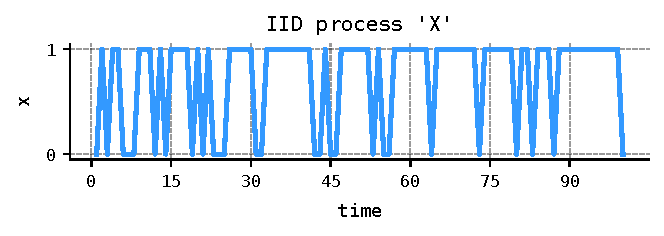
\includegraphics{images/bernoulli-trajectories.pdf}
		\caption{A trajectory of an IID process $X$ consisting of $100$ Bernoulli random variables.}
		\label{fig:bernoulli-trajectories}
	\end{subfigure}

	\begin{subfigure}{\textwidth}
		\centering
		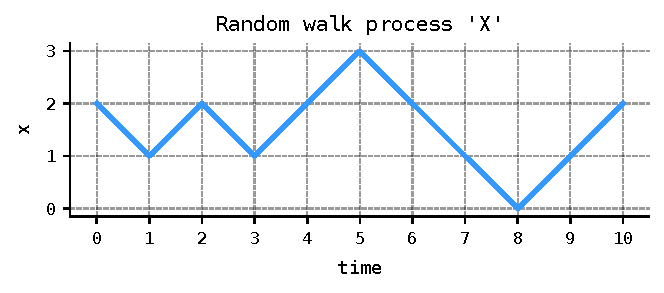
\includegraphics{images/rw-trajectories.pdf}
		\caption{A trajectory of a random walk $X$ with initial state $X_0=2$ and probability $p=0.7$ of an upward movement.}
		\label{fig:rw-trajectories}
	\end{subfigure}
	\caption{Trajectories of an IID process and a random walk. Technically, the trajectories should be visualized as sequences of dots, but for easier visualization the dots are connected with lines.}
\end{figure}

\section{Families of stochastic processes}

\subsection{Random walks}

\begin{defn}
	Let $n$ be a positive integer, $a$ a real number, and $p$ a real number in the interval $[0,1]$. A \textit{random walk} of length $n$, beginning at $a$, is a stochastic process $X$ indexed by $T = \{0,1,\ldots,n\}$ with the following properties:

	\begin{enumerate}
		\item The variable $X_0$ is deterministic, equal to $a$ for all $\omega\in \Omega$. It is called the \textit{initial state} of the random walk.
		\item The (\textit{forward}) \textit{increments}
		      \[
			      \Delta X_t \stackrel{\text{def}}{=} X_{t+1} - X_{t}, \quad t = 0,1,\ldots,n-1,
		      \]
		      are IID random variables.
		\item Each increment $\Delta X_t$ takes either the value $1$ or $-1$, the former with probability $p$ and the latter with probability $q=1-p$.
	\end{enumerate}

	If $p\neq 0.5$, the process $X$ is called a random walk \textit{with drift}; otherwise, it is called a \textit{symmetric} random walk.
\end{defn}

The ``drift'' terminology will be explained below when we plot trajectories of random walks.

\subsection{Markov processes}

\begin{defn}
	Let $(\Omega, \mathcal{F}, P)$ be a finite probability space. A stochastic process $X$ with index set $T = \{0,1,\ldots,n\}$ is called a \textit{Markov process} provided that
	\begin{equation}\label{eqn:markov}
		P(X_{t+1} \in G \mid X_0,X_1,\ldots,X_t) = P(X_{t+1} \in G \mid X_t)
	\end{equation}
	for all $t$ with $0\leq t < n$ and all Borel subsets $G\subset \mathbb{R}$.
\end{defn}

A few comments regarding the definition are in order. First, in accordance with the general definition of conditional probabilities, \eqref{eqn:markov} is an equation of \textit{random variables}. The one on the left is $\sigma(X_0,X_1,\ldots,X_t)$-measurable in general, while the one on the right is $\sigma(X_t)$-measurable. Equality of these two random variables means that they are both $\sigma(X_t)$-measurable, which is the stronger of the two measurability requirements. Second, provided that the sample space $\Omega$ is finite, there is no need to consider general Borel subsets $G$ in \eqref{eqn:markov}; indeed, in this case it is equivalent to require that
\begin{equation}\label{eqn:markov-2}
	P\left( X_{t+1} = x_{t+1} \mid X_0, \ldots,X_t \right) = P \left( X_{t+1} = x_{t+1} \mid X_t \right),
\end{equation}
for all $x_{t+1}\in \mathbb{R}$. Of course, this latter is still an equation of random variables. To verify it, it is equivalent to check the equations
\[
	P\left( X_{t+1} = x_{t+1} \mid X_0=x_0, \ldots,X_t=x_t \right) = P \left( X_{t+1} = x_{t+1} \mid X_t=x_t \right)
\]
of real numbers, one for each vector $(x_0,\ldots,x_{t+1})\in \mathbb{R}^{t+2}$.

The next theorem gives an equivalent characterization of Markov processes in terms of conditional expectations. We restrict to the case of a finite sample space so that the proof is easier, though the result is true in full generality.

\begin{thm}
	Let $X$ be a stochastic process defined on a finite probability space $(\Omega, \mathcal{F}, P)$, with index set $T = \{0,1,\ldots,n\}$. Then $X$ is Markov if and only if
	\begin{equation}\label{eqn:markov-cond}
		E\left(g(X_{t+1}) \mid X_0, X_1,\ldots,X_t\right) = E \left( g(X_{t+1}) \mid X_t \right)
	\end{equation}
	for all $t$ with $0\leq t < n$ and all functions $g: \mathbb{R} \to \mathbb{R}$.
	\begin{proof}
		For simplicity, write
		\[
			\mathcal{F}_t = \sigma\left(X_0,X_1,\ldots,X_t \right)
		\]
		for each $t$, and suppose first that the equations \eqref{eqn:markov-cond} all hold. Given a Borel subset $A\subset \mathbb{R}$ and a $t$ with $0\leq t < T$, select $g=I_A$, the indicator function of $A$. Then we compute:
		\begin{align*}
			P\left(X_{t+1} \in A \mid \mathcal{F}_t\right) & = E\left( I_{\{X_{t+1} \in A\}} \mid \mathcal{F}_t \right) \\
			                                               & = E \left( I_A(X_{t+1}) \mid \mathcal{F}_t \right)         \\
			                                               & = E \left( I_A(X_{t+1}) \mid X_t \right)                   \\
			                                               & = E \left( I_{\{X_{t+1} \in A\}} \mid X_t \right)          \\
			                                               & = P\left(X_{t+1} \in A \mid X_t\right),
		\end{align*}
		which is exactly what we wanted to show.

		Conversely, suppose that the process $X_t$ is Markov, and fix a $t$ with $0 \leq t < T$. Since $\Omega$ is finite, there are real numbers $x_1,x_2,\ldots,x_n$ such that
		\[
			X_{t+1} = \sum_{i=1}^n x_i I_{\{X_{t+1} = x_i \}}.
		\]
		If $g: \mathbb{R} \to \mathbb{R}$ is a function, then
		\[
			g(X_{t+1}) = \sum_{i=1}^n g(x_i) I_{\{X_{t+1} = x_i \}}.
		\]
		We then have:
		\begin{align*}
			E \left( g(X_{t+1}) \mid \mathcal{F}_t \right) & = \sum_{i=1}^n g(x_i) E\left(I_{\{X_{t+1} = x_i \}} \mid \mathcal{F}_t \right) \\
			                                               & = \sum_{i=1}^n g(x_i) P\left(X_{t+1} = x_i \mid \mathcal{F}_t \right)          \\
			                                               & = \sum_{i=1}^n g(x_i) P\left(X_{t+1} = x_i \mid X_t \right)                    \\
			                                               & = \sum_{i=1}^n g(x_i) E\left(I_{\{X_{t+1} = x_i \}} \mid X_t \right)           \\
			                                               & = E\left( g(X_{t+1}) \mid X_t \right),
		\end{align*}
		as desired.
	\end{proof}
\end{thm}

\section{Martingales}

\chapter{Stochastic calculus}

\section{The need for a new calculus}

In this section we continue with the discussion begun in the introduction. Our purpose is to give an informal construction of the fundamental stochastic differential equation (SDE) that characterizes \textit{diffusion processes}, whose new ingredient is a mathematical model of Brownian motion. Interpreting the solutions of the SDE will require a new type of integral belonging to stochastic calculus. In the most general setting, a careful, rigorous construction of this integral requires a good amount of measure-theoretic machinery. We leave that to the relevant textbooks; our purpose here is only to offer intuitions in the general case.

In later sections, we will specialize to the case of finite probability spaces, in which this new type of integral is a sum of random variables, Brownian motions are (approximated by) scaled random walks, and the fundamental SDE is a difference equation. All of these objects are handled by SigAlg with ease, which we will leverage to gain even more intuition.

We begin by observing a moving object. For simplicity, suppose that this object is one of the idealized ``particles'' that we encounter in textbooks on classical mechanics; that is, a so-called ``point mass,'' or a featureless speck that carries mass but lacks extension. Suppose that the motion of our particle is $1$-dimensional, along some directed axis that we use to measure lengths, distances and directions. Then, over a time interval of length $\Delta t$, our particle will have undergone a net displacement of $\Delta x$ units. The ratio of these two changes, call it $\mu$, is the average velocity of the particle over that time interval. This gives the \textit{difference} equation
\[
	\Delta x = \mu \, \Delta t.
\]

We may imagine shortening the length $\Delta t$ of the time interval while keeping the initial instant of time fixed. This will, of course, also shrink the magnitude of the net displacement $\Delta x$, and the average velocity $\mu$ will (in general) change as well. Under the idealized conditions in which it is appropriate to apply classical calculus, taken ``to the limit,'' the elapsed time $\Delta t$ transforms into its infinitesimal cousin $dt$, $\Delta x$ becomes $dx$, and the equation above is preserved, yielding the \textit{differential} equation
\begin{equation} \label{eqn:classic-diff-eq}
	dx = \mu(t) \, dt,
\end{equation}
where $\mu(t)$ is now the instantaneous velocity of the particle at the initial instant of time $t$.

To obtain the position of the particle $x(t)$ at time $t$, given its position $a = x(t_0)$ at some earlier time $t_0$ and all velocities $\mu(s)$ for $t_0 \leq s \leq t$, we integrate the differential equation:
\[
	x(t) = a + \int_{t_0}^t \mu(s) \, ds.
\]

This completes the description of the motion of a \textit{classical particle} via classical calculus. In what follows, it will be useful to refer to this particle as a \textit{deterministic} one, in the sense that its position is entirely determined at all future times $t\geq t_0$ from the velocity function $v(t)$ and its initial position. This deterministic particle contrasts with a \textit{stochastic particle}, whose infinitesimal dynamics are modeled on the classical differential equation above, but with the addition of a new term:
\begin{equation} \label{eqn:stochastic-diff-eq}
	dx = \mu(t) \, dt + \sigma(t) \, dw.
\end{equation}
The first term on the right is called the \textit{drift term}; it is carried along from the classical setting, and its role in the dynamics of the stochastic particle is no mystery. In the second term, the value $w$ is the position of a \textit{Brownian particle}: One with no drift, whose motion is entirely random, and whose mean squared displacement over any time interval equals the length of that interval. This latter particle is the idealized, mathematical avatar of one of Brown's grains of pollen. The coefficient $\sigma(t)$ is a nonnegative function of time that scales the randomness contributed by the Brownian particle. This new differential equation is an example of a \textit{stochastic differential equation} (\textit{SDE}).

And here we link up with the discussion in the introduction: If in the classical differential equation \eqref{eqn:classic-diff-eq} we are quantifying the movement of a particle by comparing its change in position $dx$ against $dt$, which is the regular and predictable (infinitesimal) time between two ticks of a clock, then in the new differential equation \eqref{eqn:stochastic-diff-eq} we are also comparing $dx$ against $dw$, which is the entirely random change in position of a Brownian particle.

Drawing inspiration from the classical case, we might then imagine that the position of the stochastic particle is obtained by integration:
\begin{equation} \label{eqn:sde-solution}
	x(t) = a + \int_{t_0}^t \mu(s) \, ds + \int_{t_0}^t \sigma(s) \, dw.
\end{equation}
The first integral on the right may be interpreted as a classical Riemann integral --- there is no issue there. The second integral on the right might be interpreted as a Riemann-Stieltjes integral, which, provided that $w$ is continuously differentiable, gives us
\begin{equation} \label{eqn:wrong-ito-integral}
	\int_{t_0}^t \sigma(s) \, dw = \int_{t_0}^t \sigma(s) w'(s) \, ds,
\end{equation}
where the integral on the right is a Riemann integral.

But there's a problem. We mentioned that the mean squared displacement of the Brownian particle over a time interval is the length of that interval. Pretending for a moment that the Brownian motion is deterministic and not random, so that we may dispense with mean values, this would imply that
\begin{equation} \label{eqn:mystery}
	(\Delta w)^2 = \Delta t.
\end{equation}
But the derivative of $w$ that appears in \eqref{eqn:wrong-ito-integral} is the limit of the ratio $\Delta w / \Delta t$ as $\Delta t \to 0$. So, to the degree that these heuristic reasonings may be trusted, we conclude that the derivative \textit{does not exist} precisely because the Brownian particle has infinite instantaneous velocity. This further implies that the differential $dw$ appearing in \eqref{eqn:stochastic-diff-eq} is a fantasy, at least in the classical sense. So, we seem to be in a jam.

In textbooks that focus more on the applications of stochastic calculus than its theoretical foundations, the SDE \eqref{eqn:stochastic-diff-eq} is left simply as informal notational shorthand that stands for \eqref{eqn:sde-solution}, and the texts instead focus their energy on making sense of the mysterious $dw$-integral. It turns out that the standard interpretation of this integral is as an \textit{Itô integral}. In the finite setting, we will see how the mysterious relation \eqref{eqn:mystery}, which seems to be one of the reasons that stochastic calculus is so different from the classical kind, is unavoidably forced on us by simple physical constraints, and we will see the discrete version of the fundamental SDE \eqref{eqn:stochastic-diff-eq} emerge naturally.



\bibliographystyle{amsplain}
\bibliography{references.bib}

\end{document}